% !TEX program = lualatex
\documentclass[aspectratio=43,professionalfonts,handout]{beamer}
\usepackage{beamer_template}

\newcommand{\LectureNum}{09}
\newcommand{\LectureTitle}{べき関数}
\newcommand{\TextPages}{p.\,88-91}
\newcommand{\NextTopic}{分数関数（１）}
\newcommand{\NextPages}{p.\,91-93}
\newcommand{\CourseName}{基礎数学B}
\renewcommand{\TermName}{前期}

\begin{document}

% -----------------------------------------------
% スライド1: 表紙＋目標＋用語・定義
% -----------------------------------------------
\begin{frame}{\CourseName\quad 第\LectureNum 回「\LectureTitle 」}
  {\small \TermName\quad \TeacherName\quad ／\quad 教科書 \TextPages\quad
  \textbf{目標}：べき関数の性質と奇関数・偶関数を理解しグラフが描ける}

  \begin{block}{用語・定義}
  \begin{description}[labelwidth=5.5em]
    \item[\kw{べき関数 y=xⁿ}] ~
    \item[\kw{奇関数}] ~
    \item[\kw{偶関数}] ~
    \item[\kw{単調増加}] ~
    \item[\kw{単調減少}] ~
  \end{description}
  \end{block}
\end{frame}

% -----------------------------------------------
% スライド2: 公式・性質
% -----------------------------------------------
\begin{frame}{公式・性質}
  \begin{block}{}
  \begin{itemize}
    \item n が奇数：奇関数・原点対称
    \item n が偶数：偶関数・y 軸対称
    \item 平行移動 y=f(x-p)+q
  \end{itemize}
  \end{block}
\end{frame}

% -----------------------------------------------
% スライド3: 図・グラフ（TikZコードを手動追加）
% -----------------------------------------------
\begin{frame}{図・グラフ}
  \centering
  % TODO: y=x³（奇）、y=x⁴（偶）、y=(x-1)⁴-2（平行移動）
  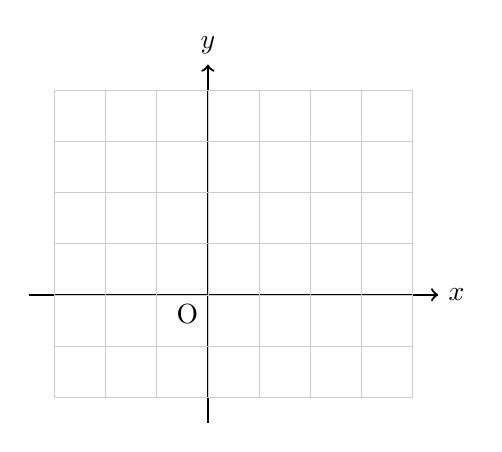
\begin{tikzpicture}[scale=0.65]
    \draw[->,thick] (-3.5,0) -- (4.5,0) node[right]{$x$};
    \draw[->,thick] (0,-2.5) -- (0,4.5) node[above]{$y$};
    \node[below left] at (0,0) {O};
    \draw[gray!40, very thin] (-3,-2) grid (4,4);
    % ここにグラフを描画
  \end{tikzpicture}
\end{frame}

% -----------------------------------------------
% スライド4: 例1→問1
% -----------------------------------------------
\begin{frame}{例1→問1}
  \begin{exampleblock}{例1・例2) p.88-89（奇偶関数の判定）}
    （板書で解説）
  \end{exampleblock}

  \vfill

  \begin{block}{問1) p.89（3問）\quad 自分で解いてみよう}
    （ノートに解くこと）
  \end{block}
\end{frame}

% -----------------------------------------------
% スライド5: 例2→問2
% -----------------------------------------------
\begin{frame}{例2→問2}
  \begin{exampleblock}{例3) p.90（グラフをかけ）}
    （板書で解説）
  \end{exampleblock}

  \vfill

  \begin{block}{問2) p.90（2問）\quad 自分で解いてみよう}
    （ノートに解くこと）
  \end{block}
\end{frame}

% -----------------------------------------------
% まとめ
% -----------------------------------------------
\begin{frame}{まとめ}
  \begin{itemize}
    \item べき関数 y=xⁿ は n が奇数なら奇関数、偶数なら偶関数
    \item 奇関数は原点対称、偶関数は y 軸対称
    \item グラフの平行移動は y=f(x-p)+q で表せる
  \end{itemize}

  \vfill
  {\small 基本問題：171, 172}
\end{frame}

\end{document}
